\documentclass{beamer} 
\usepackage{amsmath,amsthm}
\usepackage{graphicx,microtype,parskip}
\usepackage{caption,subcaption,multirow}
\usepackage{attrib}

\frenchspacing

\usetheme{default}
\usecolortheme{whale}

\setbeamertemplate{navigation symbols}{}

\setbeamercolor{title}{fg=blue,bg=white}

\setbeamercolor{block title}{fg=white,bg=gray}
\setbeamercolor{block body}{fg=black,bg=lightgray}

\setbeamercolor{block title alerted}{fg=white,bg=darkgray}
\setbeamercolor{block body alerted}{fg=black,bg=lightgray}

%\AtBeginSection[]
%{
%  \begin{frame}
%    \tableofcontents[currentsection]
%  \end{frame}
%}

\title{Cenozoic mammals and the biology of extinction}
\author{Peter D Smits}
\institute{Committee on Evolutionary Biology, University of Chicago}

\begin{document}

\begin{frame}
  \maketitle
\end{frame}

\begin{frame}
  \frametitle{Extinction}
  \begin{quotation}
    All species that have ever lived are, to a first approximation, dead.

    \tiny{\attrib{Raup 1986 \underline{The Nemesis Affair}}}
  \end{quotation}
\end{frame}

\begin{frame}
  \frametitle{Foundation}
  \begin{alertblock}{Question}
    Why do certain taxa go extinct while others do not?
  \end{alertblock}
\end{frame}

\begin{frame}
  \frametitle{In context of this study}
  \begin{block}{Rephrased}
    How does a taxon's \alert{adaptive zone} affect \alert{extinction risk?}
  \end{block}
\end{frame}

\begin{frame}
  \frametitle{Van Valen's observation}

  \begin{center}
    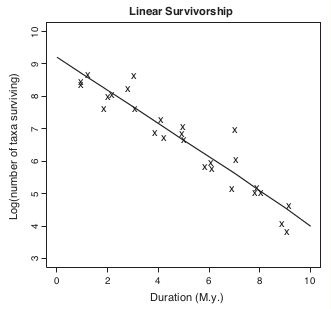
\includegraphics[height = 0.7\textheight, keepaspectratio = true]{figure/liow}

    \tiny{\attrib{Liow et al. 2011 \textit{TREE}}}
  \end{center}
\end{frame}

\begin{frame}
  \frametitle{Law of Constant Extinction}

  \begin{alertblock}{Definition}
    Extinction rate, in a given adaptive zone, is taxon--age independent.

    \tiny{\attrib{Van Valen 1973 \textit{Evol. Theory}}}
  \end{alertblock}
\end{frame}

\begin{frame}
  \frametitle{Biology and extinction}

  \begin{block}{Questions}
    \begin{itemize}
      \item Do traits related to environmental preference have different distributions of taxonomic duration? 
        \begin{itemize}
          \item Is survival best modeled by a single trait or multiple? 
          \item How do other factors, such as climate, affect these patterns? 
        \end{itemize}
      \item Is extinction taxon-age independent or dependent?
      \item Do genera and species have fundamentally different survival distributions?
    \end{itemize}
  \end{block}
\end{frame}

\begin{frame}
  \frametitle{Survival analysis}
  % analysis of time till event data
  % survival function, hazard function
  % f(t) = h(t)S(t)
  % parameterized distributions
\end{frame}

\begin{frame}
  \frametitle{Formalization of Van Valen}
  \begin{block}{Law of Constant Extinction}
    Hazard is constant with respect to time (\alert{exponential survival}).
  \end{block}

    \begin{align*}
      h(t) &= \lambda \iff S(t) = \exp^{-\lambda t}
    \end{align*}
\end{frame}

\begin{frame}
  \frametitle{Study system}
  \begin{columns}
    \begin{column}{0.5\textwidth}
      \begin{center}
        
\includegraphics[height = 0.8\textheight, width = \textwidth, keepaspectratio = true]{figure/annyong}
      \end{center}
    \end{column}
    \begin{column}{0.5\textwidth}
      \begin{itemize}
        \item Mammals
        \item Cenozoic (\(\sim 65\) My)
        \item North America, Europe, South America
        \item traits
          \begin{itemize}
            \item diet: carnivore, herbivore, omnivore, insectivore
            \item locomotion: \\ground dwelling, \\arboreal, scansorial
            \item body size
          \end{itemize}
      \end{itemize}
    \end{column}
  \end{columns}
\end{frame}

\begin{frame}
  \frametitle{Approach}
  \begin{columns}
    \begin{column}{0.5\textwidth}
      
    \end{column}<++>
  \end{columns}<++>
\end{frame}

\begin{frame}
  \frametitle{Acknowledgements}
  \begin{columns}
    \begin{column}{0.5\textwidth}
      \begin{itemize}
        \item \textbf{Committee}
          \begin{itemize}
            \item Kenneth D. Angielczyk (co-advisor)
            \item Michael J. Foote (co-advisor)
            \item P. David Polly
            \item Richard H. Ree
          \end{itemize}
        \item Discussion
          \begin{itemize}
            \item David Bapst, Megan Boatright, Ben Frable, Colin Kyle, Darcy Ross, Liz Sander
            \item John Alroy, Graeme Lloyd, Carl Simpson, Graham Slater
          \end{itemize}
      \end{itemize}
    \end{column}
    \begin{column}{0.5\textwidth}
      
\includegraphics[height = 0.3\textheight, keepaspectratio = true]{figure/chicago} \\
      
\includegraphics[height = 0.3\textheight, width = 0.5\textwidth, keepaspectratio = true]{figure/field} \\
    \end{column}
  \end{columns}
\end{frame}

\appendix

\begin{frame}
  \frametitle{Differential preservation and survival}

  \begin{columns}
    \begin{column}{0.5\textwidth}
      \begin{center}
        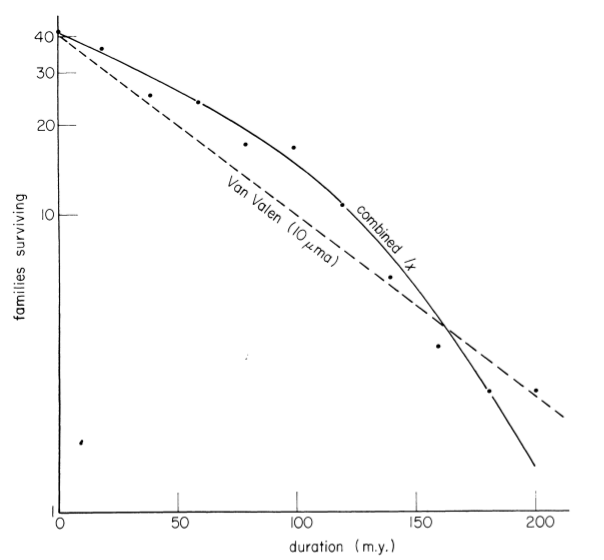
\includegraphics[height = 0.4\textheight, width = \textwidth, keepaspectratio = true]{figure/raup}

        \tiny{\attrib{Raup 1975 \textit{Paleobio.}}}

        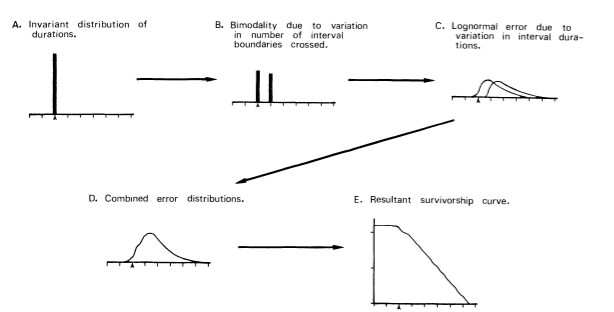
\includegraphics[height = 0.4\textheight, width = \textwidth, keepaspectratio = true]{figure/sepkoski}

        \tiny{\attrib{Sepkoski 1975 \textit{Paleobio.}}}
      \end{center}
    \end{column}
    \begin{column}{0.5\textwidth}
      two groups in four scenarios
      \begin{itemize}
        \item \(=\) birth, death; \\\(=\)preservation
        \item \(=\) birth, death; \\\(!=\)preservation
        \item \(!=\) birth, death; \\\(=\) preservation
        \item \(!=\) birth, death; \\\(!=\)preservation
      \end{itemize}
    \end{column}
  \end{columns}
\end{frame}

% any preliminary results?

\end{document}
